\subsection{Methods}
% -------------------------------------------------------------------------
A typical watershed segmentation is performed to determine if a difficult
segmentation can take advantage of one of the previously mentioned
marker generating methods, based on whether segmenting based on distance
transform maxima results in over- or under-segmentation.
In a typical watershed
segmentation routine, an image is semantically segmented and represented
as a binary image, the binary
image undergoes a distance transformation, and the maxima of the distance
transformation is used to generate markers to seed the watershed
segmentation. This type of routine is tested with an image of sand grains
to see if the resulting segmentation meets expectations for an image of
irregularly-shaped, multi-sized, and tightly-clustered sand grains
(\ref{fig/05/raw-bw}.a). This image is loaded from file using the
Python package \textit{imageio} and converted to a \textit{NumPy}
array \cite{imageio,numpy}. As an array, the image is
binarized using the Otsu thresholding algorithm
implemented in \textit{scikit-image} (\ref{fig/05/raw-bw}.b)
\cite{Otsu1979,skimage}.

\begin{figure}[ht]
    \centering
    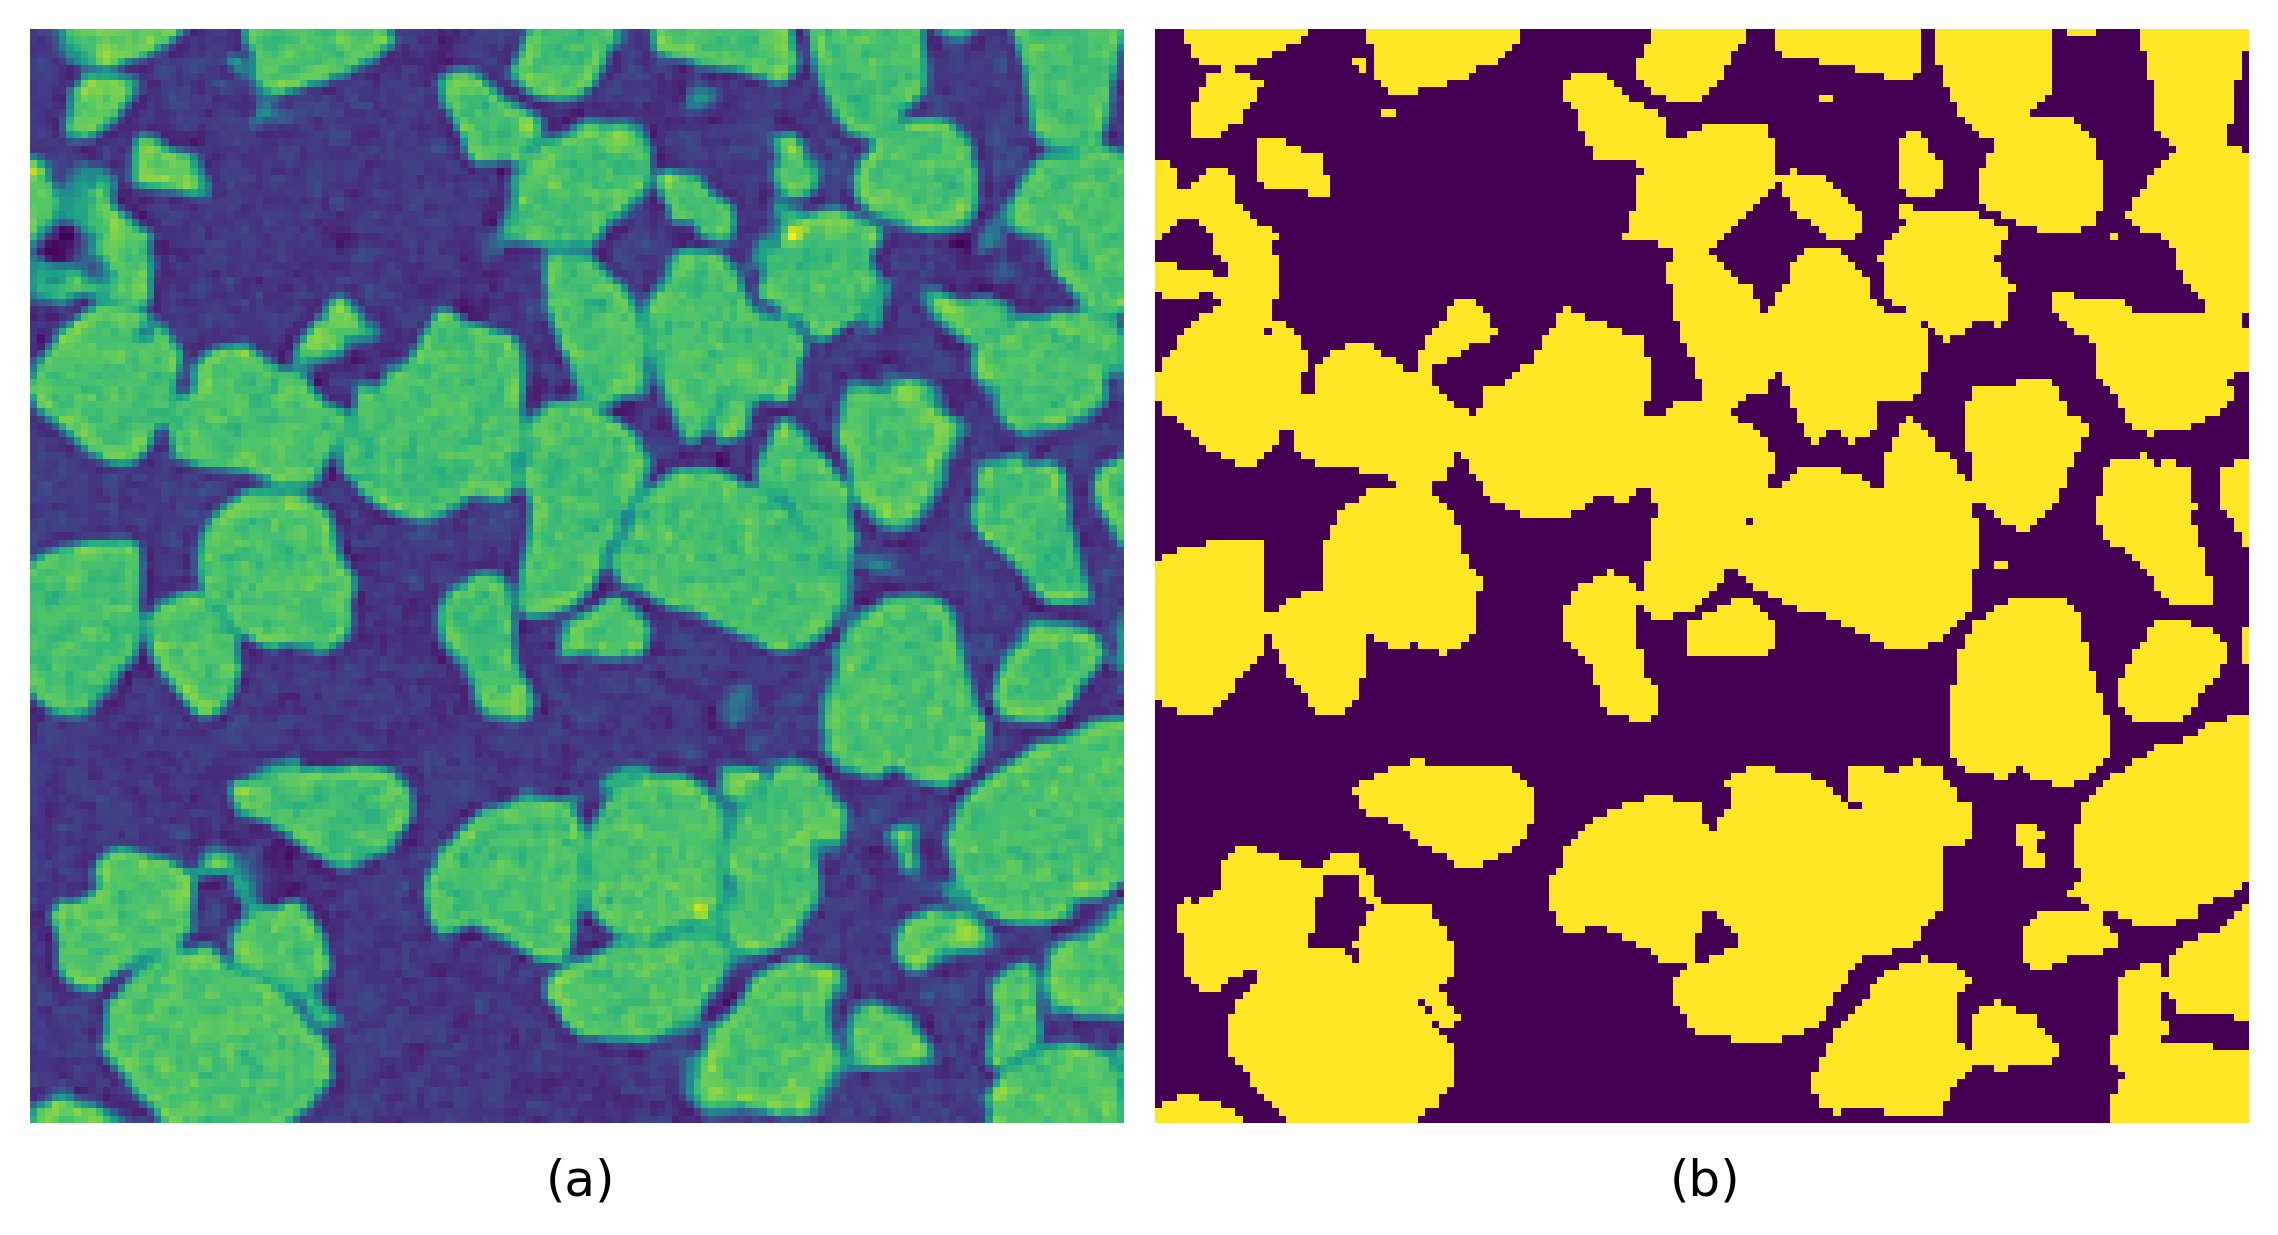
\includegraphics[width=0.75\textwidth]{figures/05/01-raw-bw.png}
    \caption{
        \small\setstretch{1}
        (a) Raw image depicting sand particles sliced from a 3D CT scan.
        (b) Binary image created from the raw image with Otsu thresholding.
        Yellow regions represent foreground pixels (valued one) while purple
        regions represent background pixels (valued zero).
    }
    \label{fig/05/raw-bw}
\end{figure}

After creating the binary image, a series of markers are generated which
will be used to seed the watershed segmentation. The distance of each
foreground pixel to the nearest background pixel calculated using the
Euclidean distance transformation implemented in \textit{SciPy} \cite{scipy}.
This distance
transformation is inverted to pass to the watershed algorithm. The local
maxima of this distance transform (equivalent to the local minima of the
inverted distance transformation) correspond to the points farthest from
the edges of the binary image (\ref{fig/05/typical}.b).
In the case of some of the
oblong particles present in the image, detecting all the local minima
resulted in connected groups of redundant minima where multiple
neighboring pixels exist at the same distance from the edge of the binary
image. This was addressed by using the \textit{scikit-image} functions
\textit{label} and \textit{regionprops} to retain only the centermost
point of connected minima. Once disconnected and non-redundant minima
were obtained, these points were used as markers to seed a watershed
algorithm implemented in \textit{scikit-image}.
The resulting segmented regions (\ref{fig/05/typical}.c) do not meet
expectations based on the visually discernible particles in the original
image. Since the segmented regions are over-segmented in some places and
under-segmented in others, the methods from literature outlined previously
cannot correct the segmentation.

\begin{figure}[ht]
    \centering
    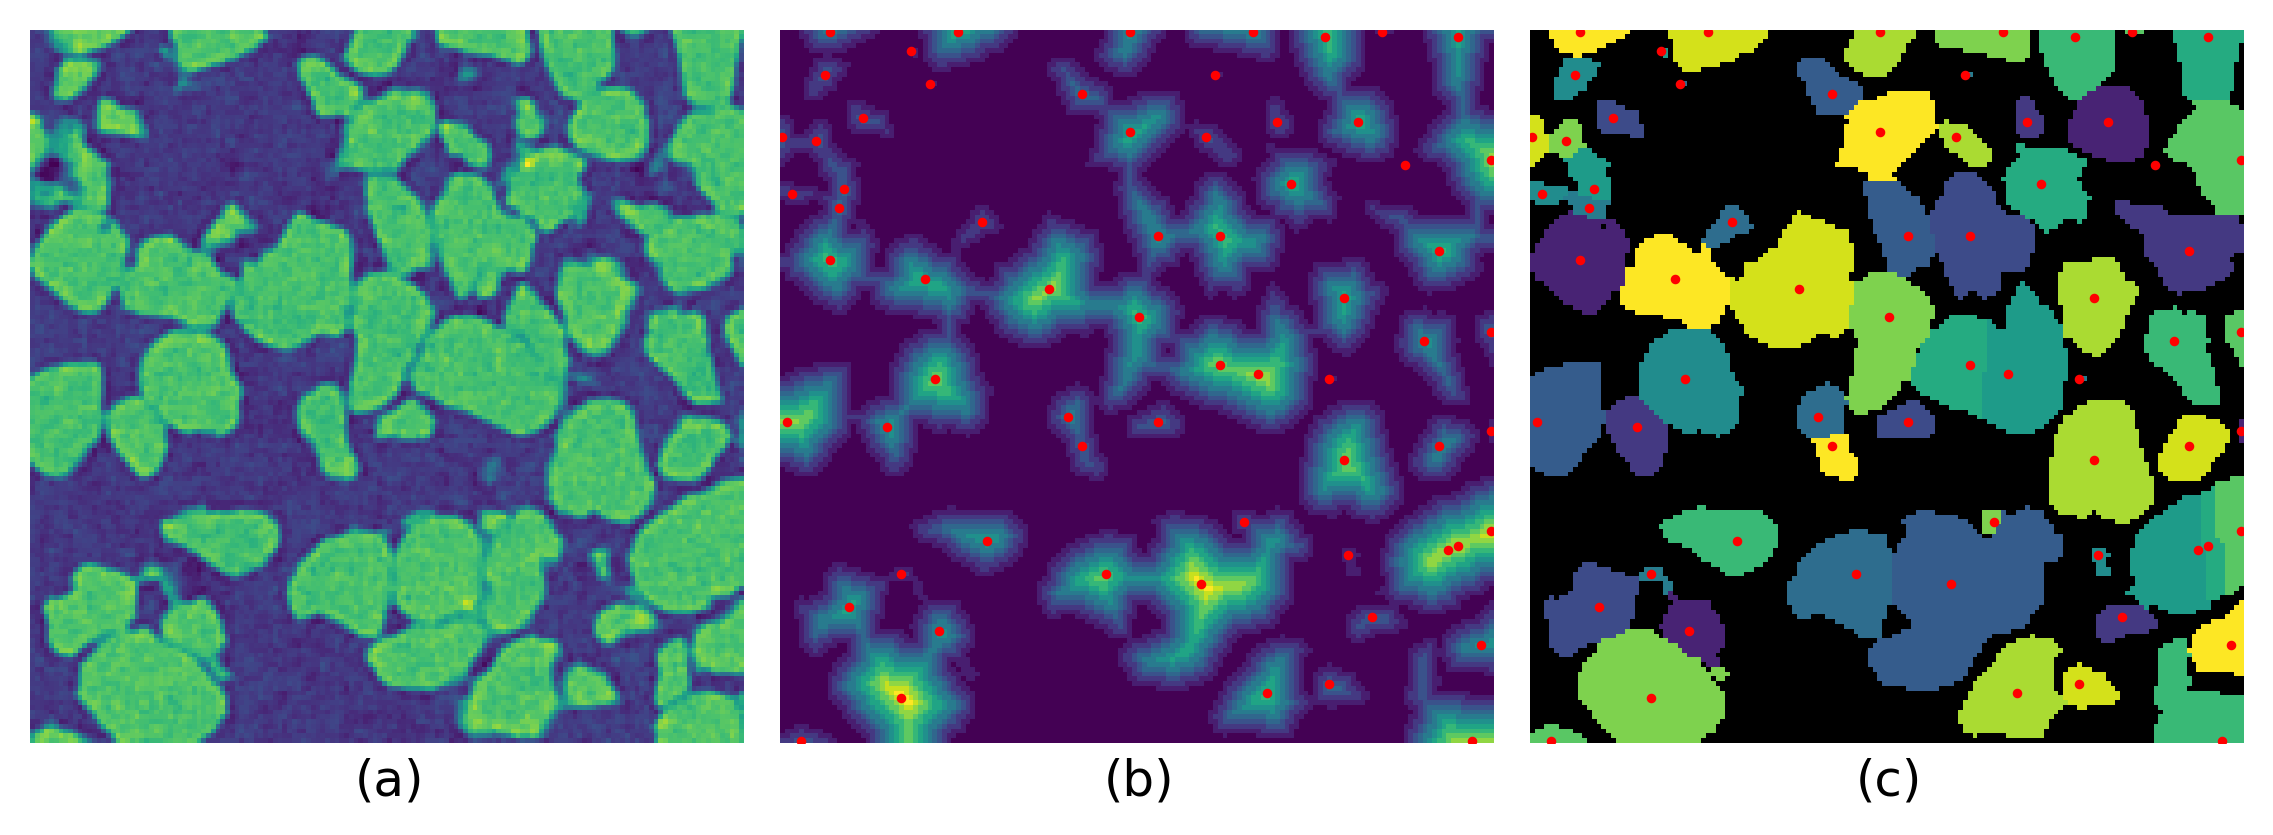
\includegraphics[width=0.75\textwidth]{figures/05/02-typical-routine.png}
    \caption{
        \small\setstretch{1}
        (a) Image depicting sand particles sliced from a 3D CT scan.
        (b) Euclidean distance transformation of Otsu-binarized image
        (\ref{fig/05/raw-bw}.b) with local maxima denoted by red points.
        (c) Watershed segmentation of inverted Euclidean distance
        transformation seeded by local minima of the inverted distance
        transformation (red points).
    }
    \label{fig/05/typical}
\end{figure}

% -------------------------------------------------------------------------
\subsubsection{Adding a Preprocessing Routine to Generate New Markers}
% -------------------------------------------------------------------------
To achieve segmentation results that align more closely with expectations,
the strategy of the procedure outlined in this work is to first create a set
of markers to intentionally over-segment the image, followed by a
subsequent step of determining region neighbors and correcting the
over-segmentation by merging neighboring regions
according to edge strength. This will ensure there is not a combination of
over- and under-segmentation occurring. New markers are needed
to achieve this over-segmentation such that each particle in the original
image contains at least one marker to prevent under-segmentation.
A preprocessing routine is employed to
generate these markers. The original image is rescaled between the 5th and
95th percentiles (\ref{fig/05/routine}.b).
Histogram equalization from \textit{scikit-image} is
performed on the rescaled image to enhance the intensities of the maxima
within the particles (\ref{fig/05/routine}.c).
Histogram equalization spreads out the values of the image
across the entire range, allowing for the creation of a binary image that
contains only the innermost regions of the particles. To create this
binary image, the multiple-class functionality of Otsu's method
implemented in \textit{scikit-image} is used to separate the image into three
classes. This can be visualized as a ternary image
(\ref{fig/05/routine}.d), however
only the regions above the uppermost threshold value are selected to
create the binary image. Holes within the created regions are filled using
the function \textit{binary\textunderscore fill\textunderscore holes}
from the multidimensional image processing
submodule in \textit{SciPy} (\ref{fig/05/routine}.e).
This maximizes the distances calculated via
distance transformation operating on the multi-Otsu binary image
(\ref{fig/05/routine}.f). The local maxima of this distance
transformation are useful for this
routine because they over-represent the particles in the image
(i.e., more markers than particles), which will result in the
over-segmentation desired at this stage of the procedure.

\begin{figure}[ht]
    \centering
    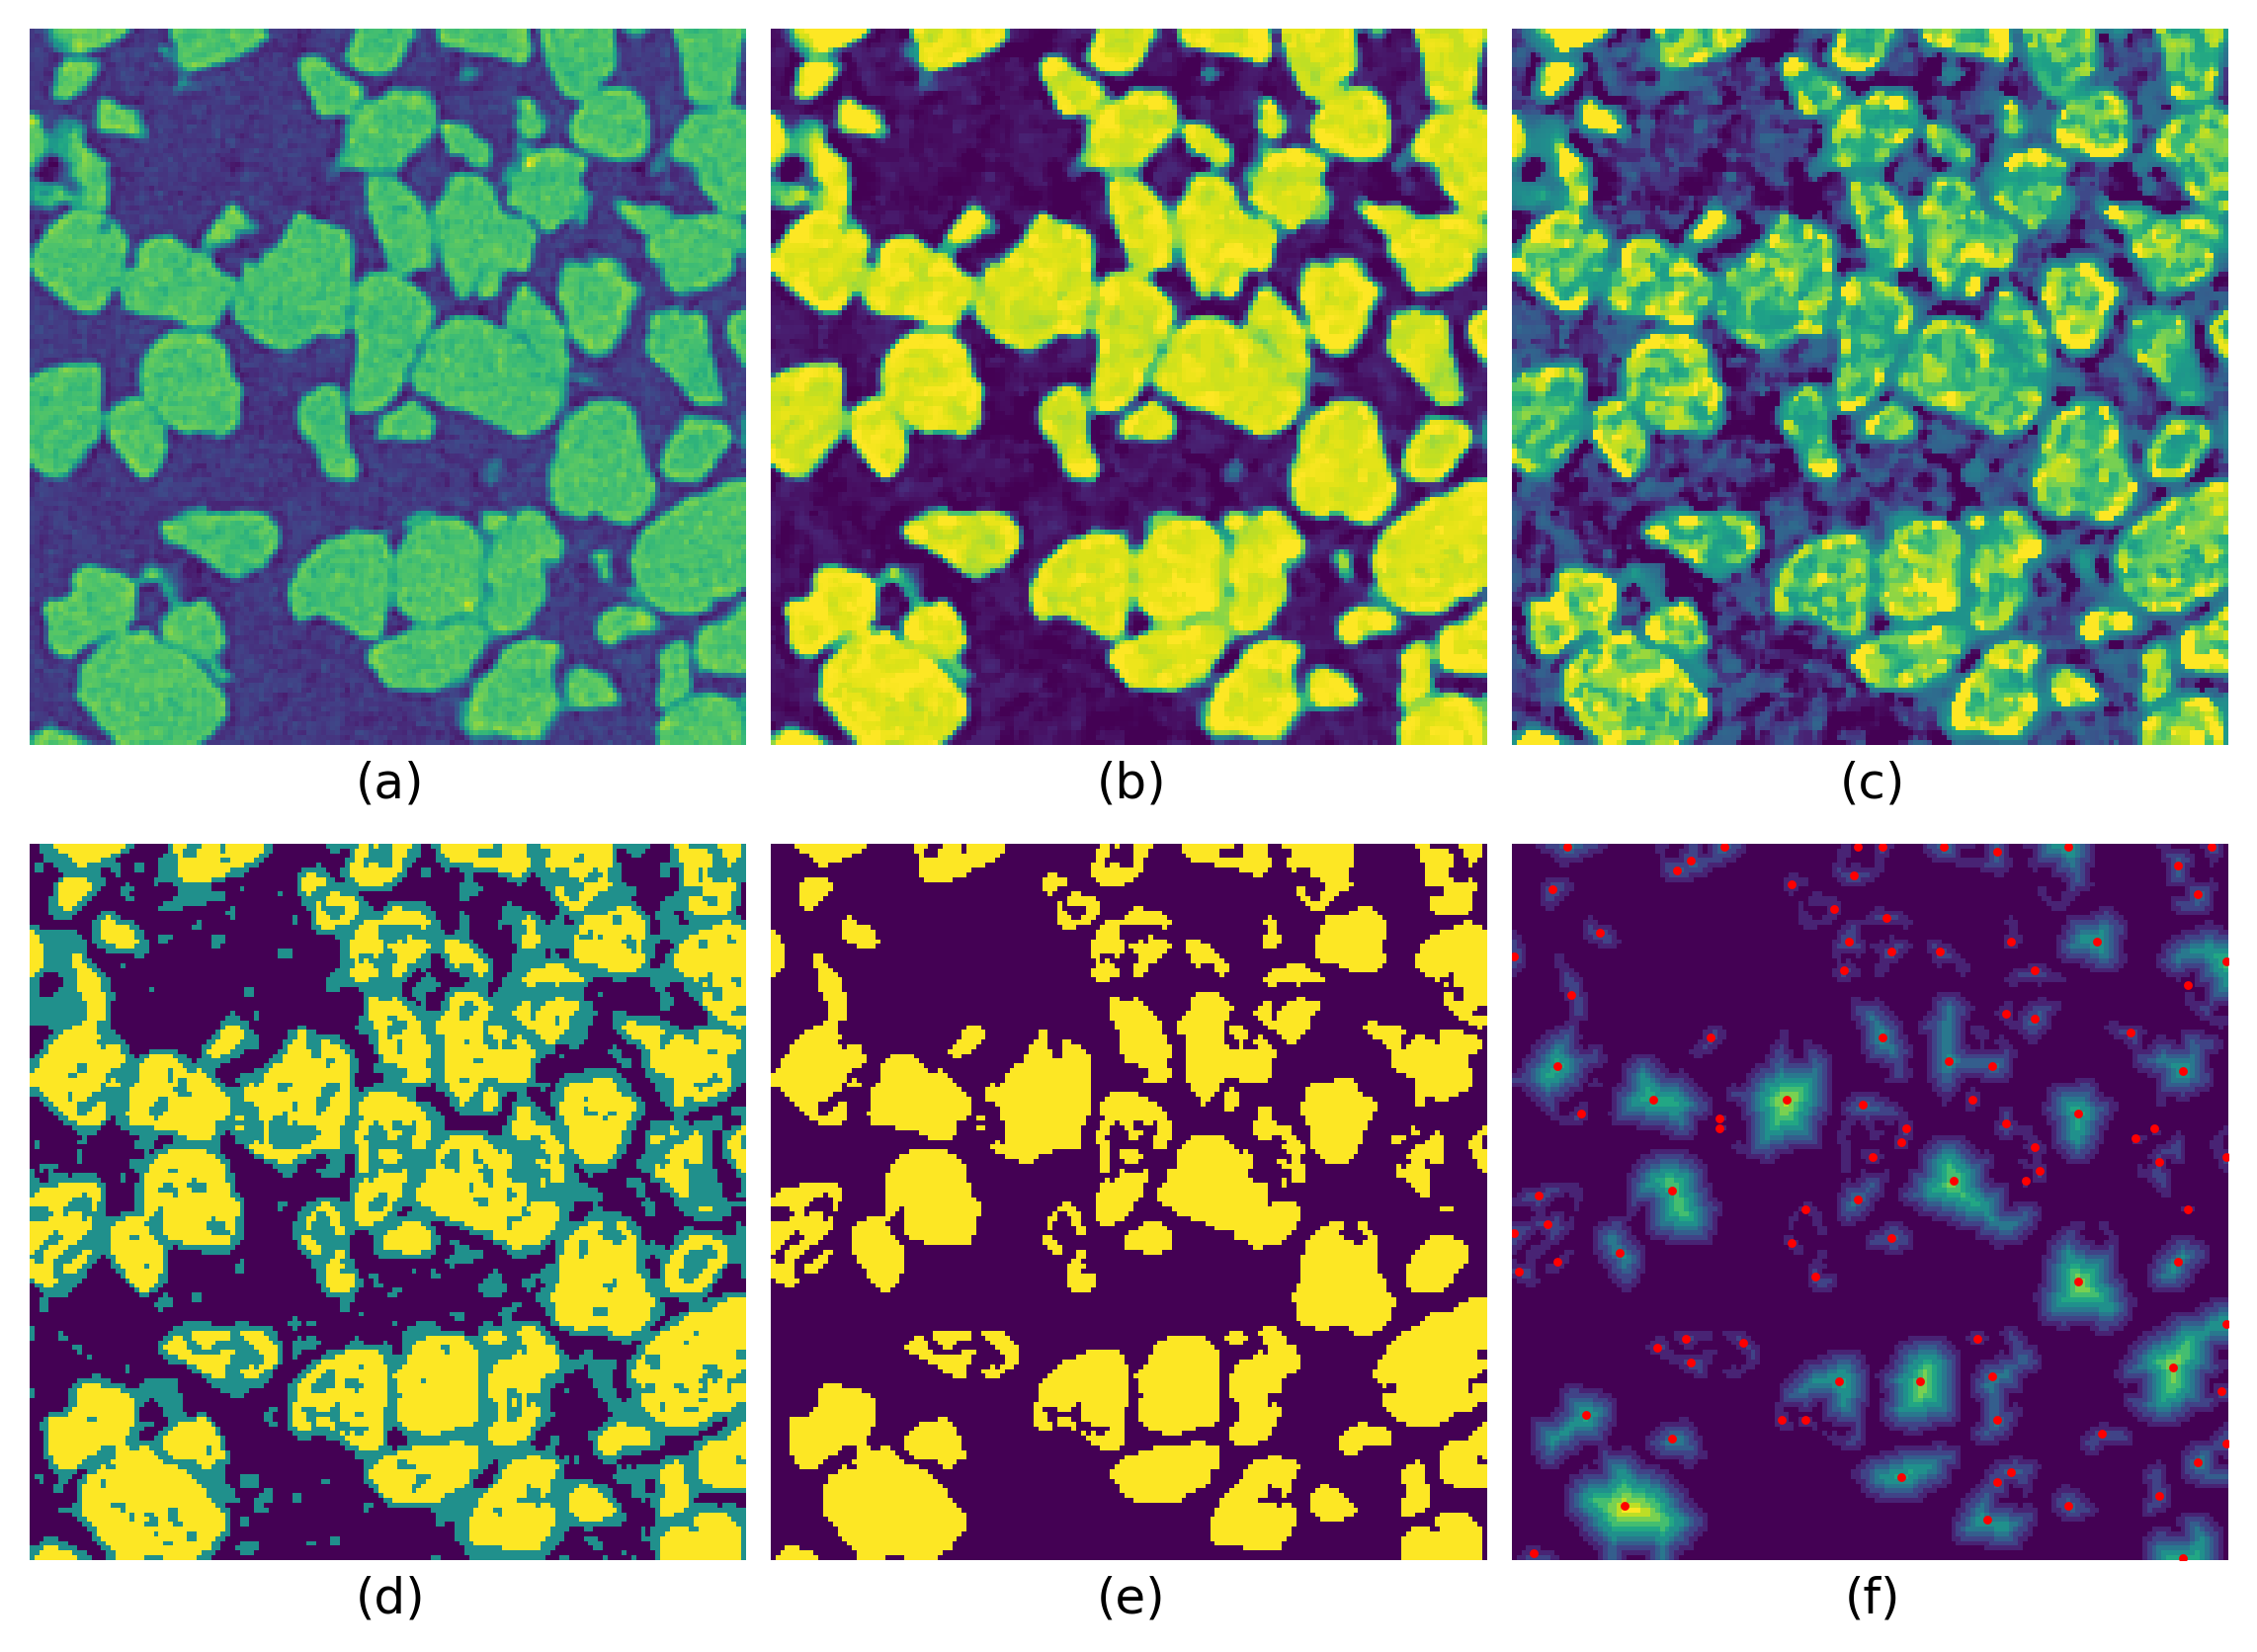
\includegraphics[width=0.75\textwidth]{figures/05/03-routine.png}
    \caption{
        \small\setstretch{1}
        (a) Image depicting sand grains sliced from a 3D CT scan.
        (b) Image rescaled to the range defined by the 5th and 95th percentile
        intensities.
        (c) Rescaled image after histogram equalization to enhance
        maxima within the particles.
        (d) Histogram-equalized image converted into
        a ternary image following application of a multi-Otsu algorithm with
        three classes.
        (e) Binary image created by thresholding the with uppermost value
        calculated by multi-Otsu algorithm. All holes within resulting regions
        of binary image are filled.
        (f) Euclidean distance transformation of multi-Otsu binary image with
        local maxima denoted by red points.
    }
    \label{fig/05/routine}
\end{figure}

% -------------------------------------------------------------------------
\subsubsection{Preparing Over-Segmentation}
% -------------------------------------------------------------------------
Before the local maxima markers are used to seed a watershed segmentation,
the markers are filtered such that any points close to a particle edge
in the image are removed. Over-segmented regions will be merged according
to edge strength between the markers, so having a marker lie on
an edge between two particles may prevent the edge from being detected. To
remove the markers closest to edges, an image is created that enhances the
intensity of particle edges by applying a Sobel filter, implemented in
\textit{scikit-image}, to the rescaled image (\ref{fig/05/edges}.b)
\cite{Kanopoulos1988}. In this image, the
strongest edges are represented by the highest intensities in the image.
The edges in the Sobel-filtered image are further emphasized by performing
adaptive histogram equalization from \textit{scikit-image}, which increases
the intensity of the weaker edges between particles.

\begin{figure}[ht]
    \centering
    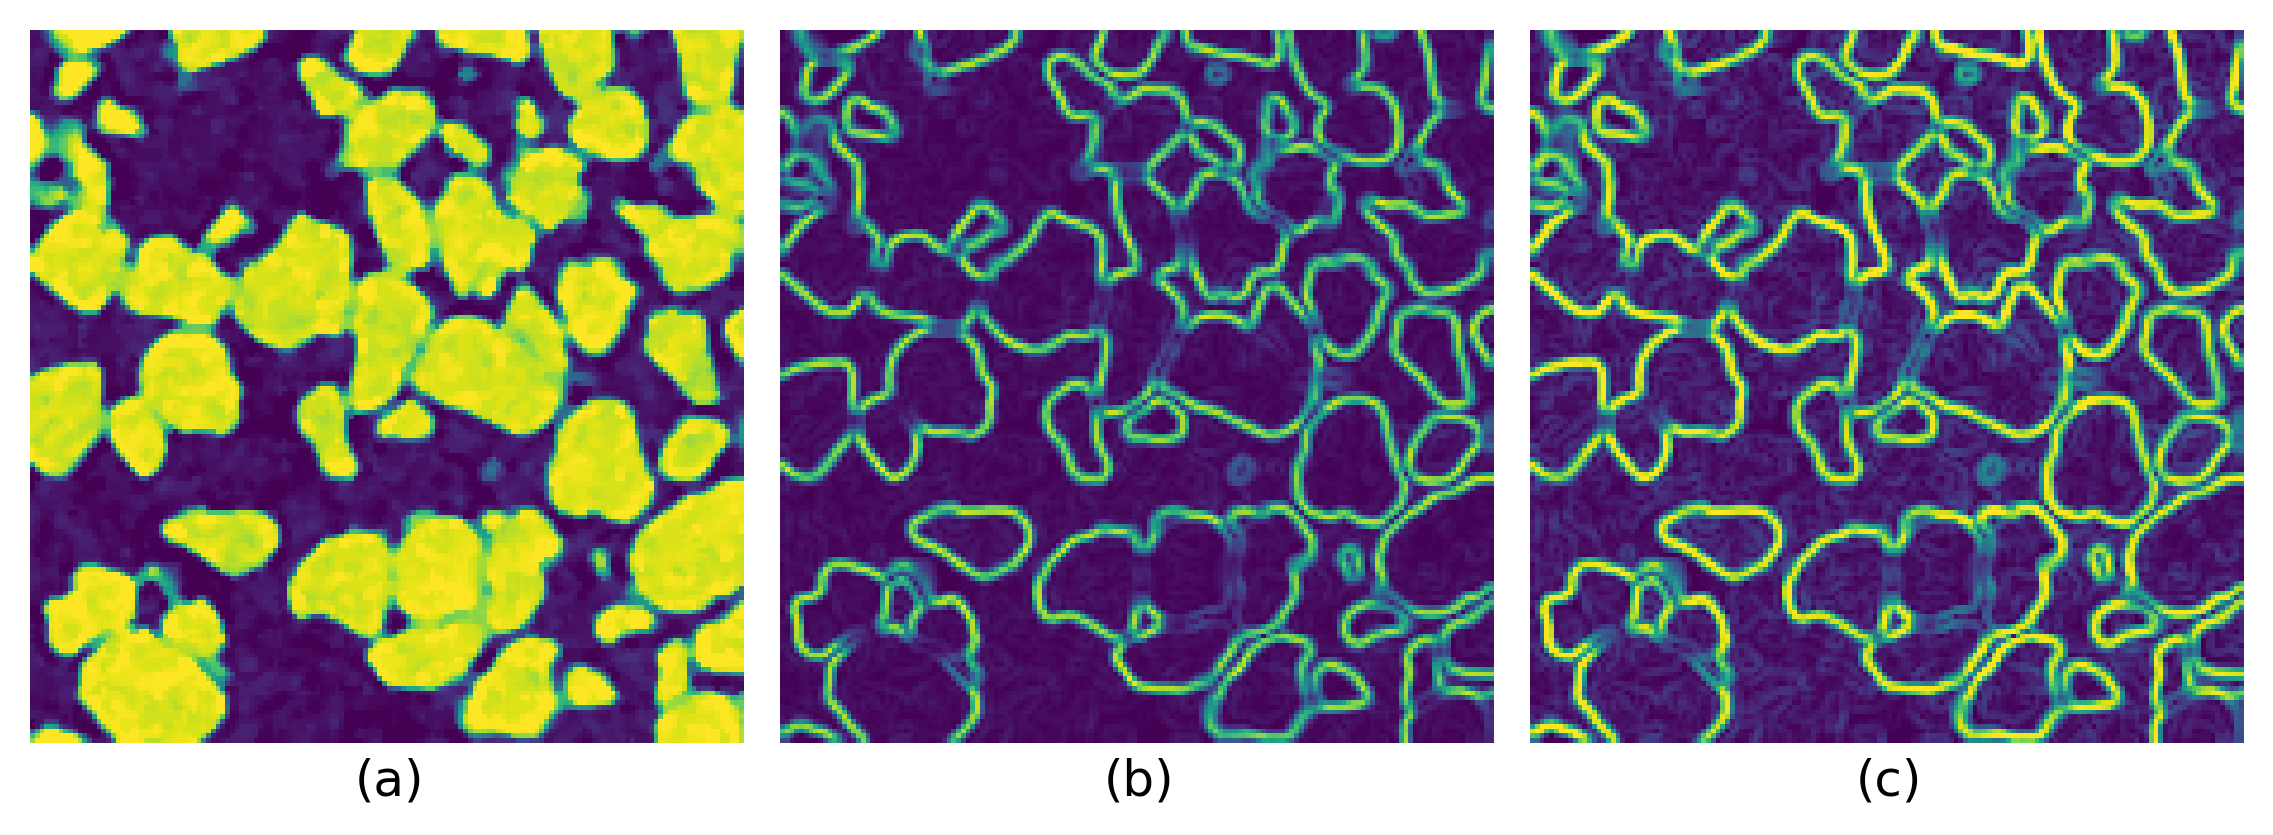
\includegraphics[width=0.75\textwidth]{figures/05/04-edges.png}
    \caption{
        \small\setstretch{1}
        (a) Rescaled image depicting sand grains
        (\ref{fig/05/routine}.b).
        (b) Rescaled image after application of a Sobel filter to enhance the
        edges of particles within the image.
        (c) Sobel-filtered image after adaptive histogram equalization is
        performed to further enhance particle edges.
    }
    \label{fig/05/edges}
\end{figure}

Sampling the intensity of the edge image (\ref{fig/05/edges}.c) at
the locations of
the inverse distance transformation minima, the points closest to the
edges will have the highest intensity. The points with intensities above
the 95th percentile are removed (\ref{fig/05/seeds}.b). The remaining
minima will be used as markers to seed the watershed segmentation.

\begin{figure}[ht]
    \centering
    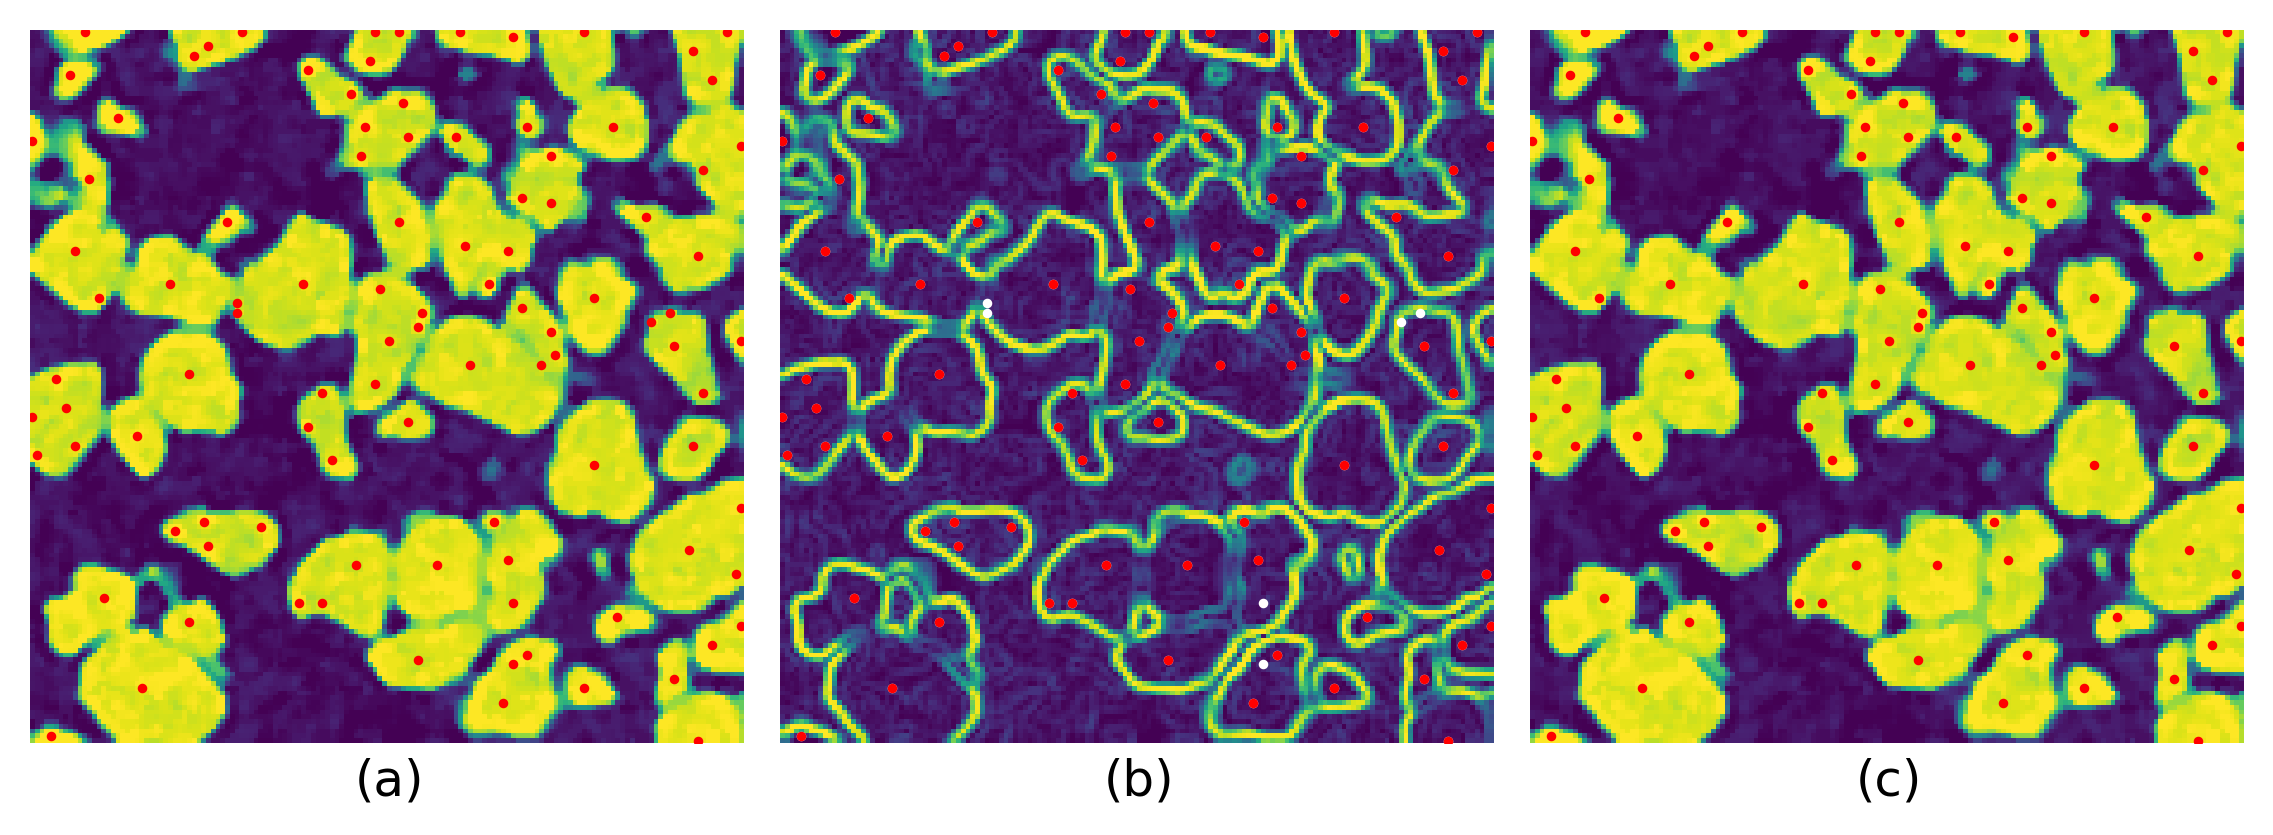
\includegraphics[width=0.75\textwidth]{figures/05/05-seeds.png}
    \caption{
        \small\setstretch{1}
        (a) Rescaled image depicting sand grains overlaid with
        inverted distance transformation minima in red.
        (b) Edge image (\ref{fig/05/edges}.c) with minima overlaid.
        White points are removed by filtering process for being too close
        to the particle edges while red points will be used as markers for
        the watershed segmentation.
        (c) Edge-filtered local minima (red) overlaid on the rescaled image.
    }
    \label{fig/05/seeds}
\end{figure}

The filtered markers seed a watershed segmentation operating on the
inverted distance transformation (\ref{fig/05/overseg}.b) created from
the multi-Otsu-binarized image (\ref{fig/05/routine}.e). Compared to the
visually discernible sand grains in the raw image (\ref{fig/05/overseg}.a),
the results of the watershed segmentation appear over-segmented as desired for
this stage of the procedure (\ref{fig/05/overseg}.c).

\begin{figure}[ht]
    \centering
    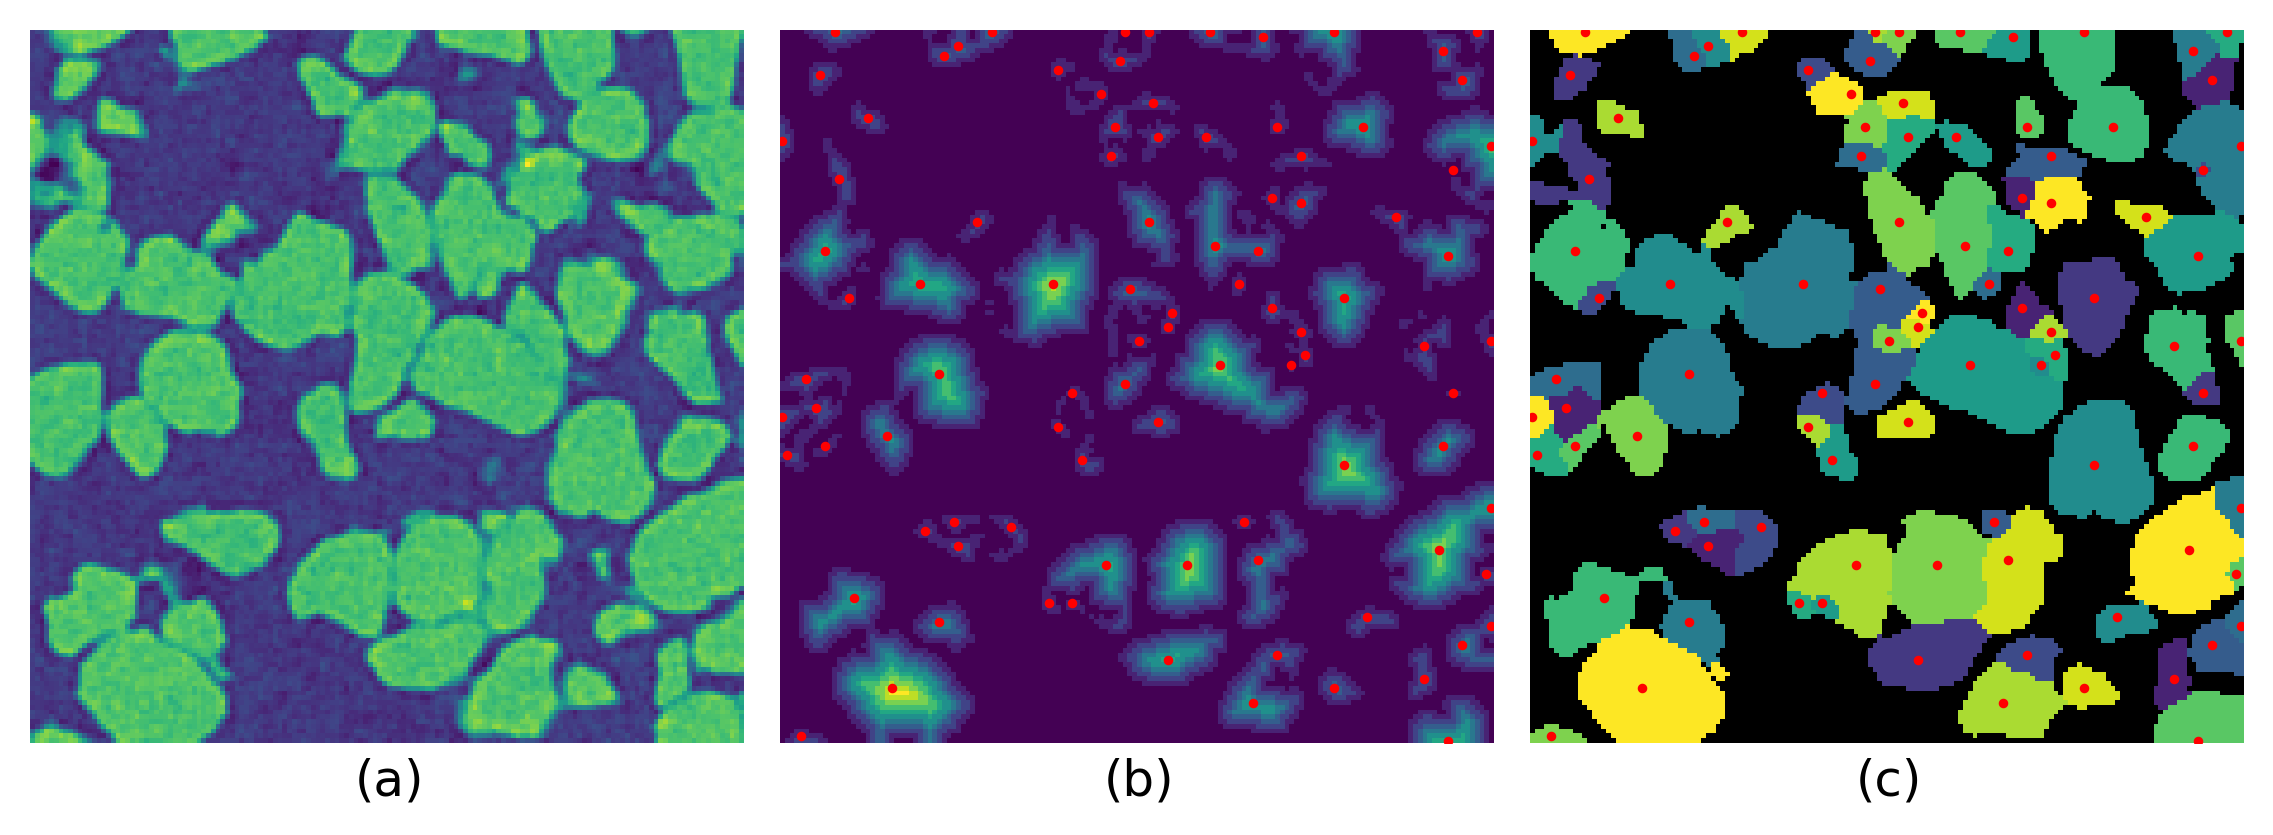
\includegraphics[width=0.75\textwidth]{figures/05/06-overseg.png}
    \caption{
        \small\setstretch{1}
        (a) Image depicting sand grains to be segmented.
        (b) Euclidean distance transformation of multi-Otsu-binarized image
        (\ref{fig/05/routine}.e) with edge-filtered local maxima denoted
        by red points.
        (c) Watershed segmentation results of the inverted Euclidean distance
        transformation seeded by the edge-filtered local maxima in previous
        image.
    }
    \label{fig/05/overseg}
\end{figure}

% -------------------------------------------------------------------------
\subsection{Delaunay Triangulation to Connect Markers and Detect Edges}
% -------------------------------------------------------------------------
A method has been developed to merge the over-segmented regions according
to edges detected in the vicinity of the regions.
Locations
between two regions determined to be neighbors must be searched for edges.
The regions will be merged if an edge is not detected between the two
regions. Before this can happen, however, a method is needed for
determining neighboring regions.
Each marker used to seed the segmentation will correspond
to one region, so the markers can be used to determine region neighbors,
but this process is still nontrivial.
As multi-sized markers will have neighbors at varying
distances, a method is needed that will connect each marker to its
neighboring markers without prior information about the distance to
those neighboring markers.
This can be achieved using Delaunay triangulation,
which calculates triangles between a distribution of points such that no
other points are within the circumcircle each triangle creates
\cite{Voronoi1908,Delaunay1934,Aurenhammer1991}.
The result is a structure that connects points with line segments of
varying lengths that do not overlap. Delaunay triangulation has been
applied to image segmentation before as an alternative method to watershed
segmentation. Wen et. al use Delaunay triangulation to segment clumps of
nuclei in cell-based fluorescent imaging \cite{Wen2009}.
In their method, points of
high curvature are detected in an image. These points are connected via
Delaunay triangulation and a geometry constraint is applied to the
triangulated lines to select the lines that separate the nuclei.
The method achieves results that align with expectations, however an
important requirement for this success is the consistently round shape
of the segmented nuclei such that
points of high curvature in the binary
image only occur at the points of contact between the particles.
Due to the irregular shape of the sand particles in the present work,
there are high points of curvature around the perimeter of single sand
grains, not only where the grains are in contact,
so this method would not be effective.
Instead of trying to use Delaunay
triangulation as a replacement for watershed segmentation, the routine
presented in this work uses Delaunay triangulation to
assist in merging over-segmented regions.

The neighbors of each marker are determined by calculating a
Delaunay triangulation with \textit{SciPy}, using the markers
corresponding to over-segmented regions (\ref{fig/05/delaunay}.a)
as the input vertices. The resulting
network of lines connect each marker to neighboring markers
(\ref{fig/05/delaunay}.b). This is useful in the
context of irregularly-shaped and multi-sized particles because the lines
connecting neighboring markers can be drastically different lengths.
Sampling the intensity of the edge image along each of these lines yields
intensity profiles, analysis of which is used to define the edge
detection. With a robust enough definition of a detected edge, edges can
even be detected between tightly-clustered sand grains. In this work,
an edge is defined as detected between two neighboring markers if the
maximum intensity along the line connecting the markers satisfies two
conditions: (1) the maximum intensity along the line must be greater than
10 percent of the edge image global maximum, and (2) the maximum
intensity along the line must not occur at either end of the line.
Most strongly defined
edges in the image are near the edge image global maximum, but the edge
detection definition must encompass a larger range of values to capture
the weakly defined edges which have a much lower intensity. Since this
edge detection value is so low, some lines that don't cross any edges are
falsely flagged as crossing an edge. This typically happens when one or
both markers at either end of the line are near particle edges, hence
the necessity of the second condition. The number
of falsely flagged edges is reduced by ignoring detected edges when the
maximum intensity of the line occurs at either endpoint. Markers that are
connected by lines on which edges are not detected are defined as
belonging in the same ``particle neighborhood'' and are merged in the
final stage of the procedure. The criteria used here for forming these
particle neighborhoods were
determined based on observation of the edges in this image and could be
tailored to specific experiments.

\begin{figure}[ht]
    \centering
    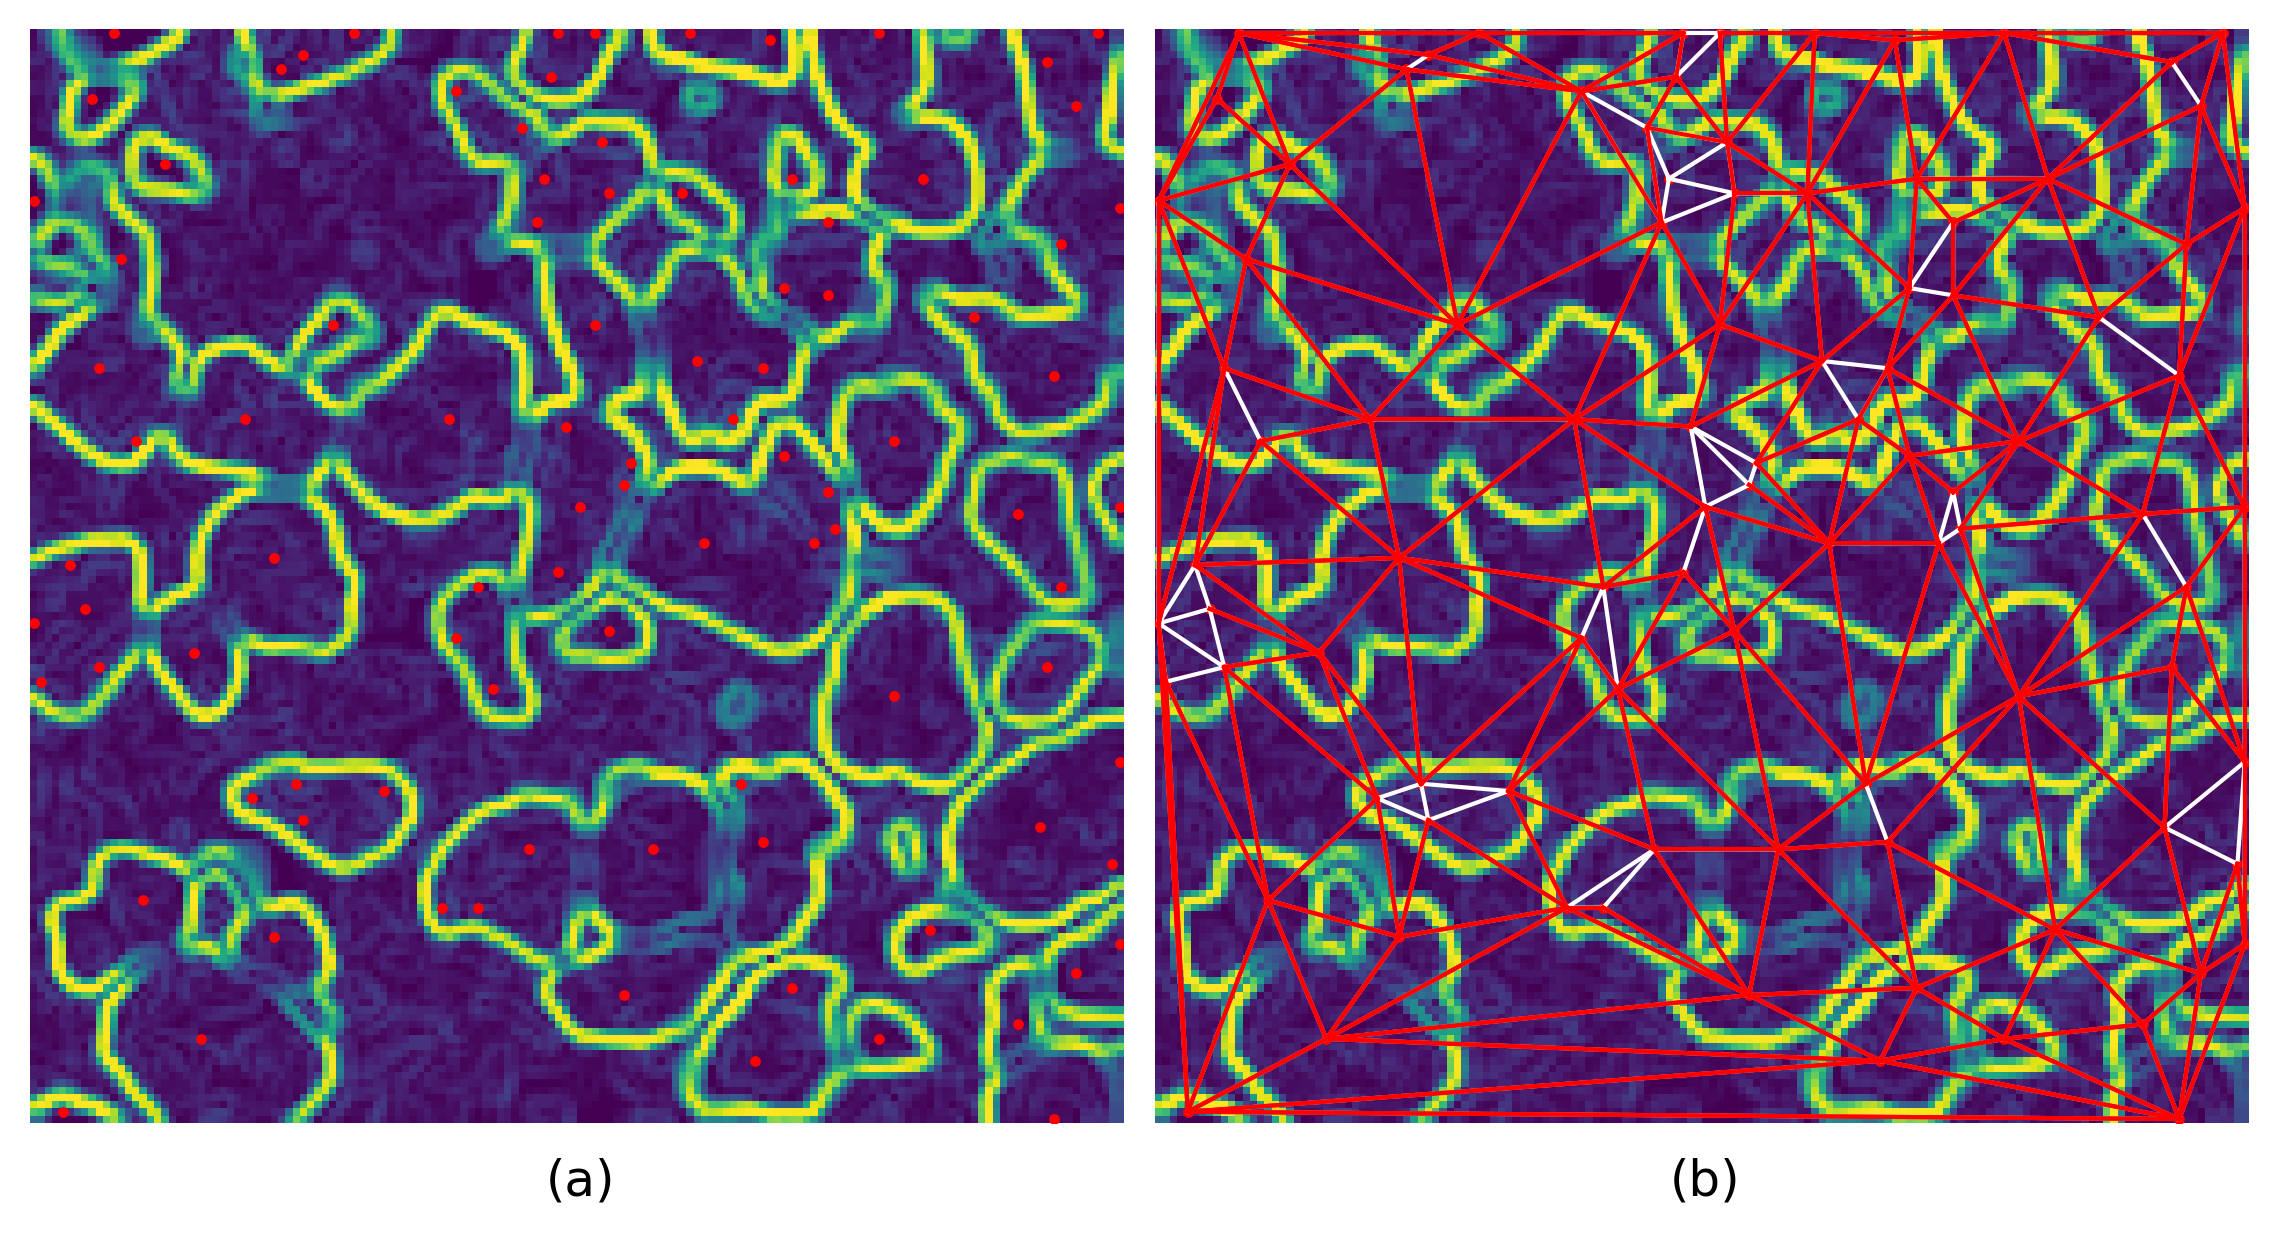
\includegraphics[width=0.75\textwidth]{figures/05/07-delaunay.png}
    \caption{
        \small\setstretch{1}
        (a) Edge-filtered maxima used as markers (red) overlaid on the
        edge image (\ref{fig/05/edges}.c).
        (b) Edge image overlaid with Delaunay
        triangulation. Red lines denote lines across which an edge was detected
        while white lines denote lines across which no edges were detected.
        Markers connected by white lines are defined as existing in the same
        ``particle neighborhood''.
    }
    \label{fig/05/delaunay}
\end{figure}

